\documentclass{beamer}
\mode<presentation>
\usepackage{amsmath}
\usepackage{amssymb}
%\usepackage{advdate}
\usepackage{adjustbox}
\usepackage{subcaption}
\usepackage{enumitem}
\usepackage{multicol}
\usepackage{mathtools}
\usepackage{listings}
\usepackage{url}
\def\UrlBreaks{\do\/\do-}
\usetheme{Boadilla}
\usecolortheme{lily}
\setbeamertemplate{footline}
{
  \leavevmode%
  \hbox{%
  \begin{beamercolorbox}[wd=\paperwidth,ht=2.25ex,dp=1ex,right]{author in head/foot}%
    \insertframenumber{} / \inserttotalframenumber\hspace*{2ex} 
  \end{beamercolorbox}}%
  \vskip0pt%
}
\setbeamertemplate{navigation symbols}{}

\providecommand{\nCr}[2]{\,^{#1}C_{#2}} % nCr
\providecommand{\nPr}[2]{\,^{#1}P_{#2}} % nPr
\providecommand{\mbf}{\mathbf}
\providecommand{\pr}[1]{\ensuremath{\Pr\left(#1\right)}}
\providecommand{\qfunc}[1]{\ensuremath{Q\left(#1\right)}}
\providecommand{\sbrak}[1]{\ensuremath{{}\left[#1\right]}}
\providecommand{\lsbrak}[1]{\ensuremath{{}\left[#1\right.}}
\providecommand{\rsbrak}[1]{\ensuremath{{}\left.#1\right]}}
\providecommand{\brak}[1]{\ensuremath{\left(#1\right)}}
\providecommand{\lbrak}[1]{\ensuremath{\left(#1\right.}}
\providecommand{\rbrak}[1]{\ensuremath{\left.#1\right)}}
\providecommand{\cbrak}[1]{\ensuremath{\left\{#1\right\}}}
\providecommand{\lcbrak}[1]{\ensuremath{\left\{#1\right.}}
\providecommand{\rcbrak}[1]{\ensuremath{\left.#1\right\}}}
\theoremstyle{remark}
\newtheorem{rem}{Remark}
\newcommand{\sgn}{\mathop{\mathrm{sgn}}}
\providecommand{\abs}[1]{\left\vert#1\right\vert}
\providecommand{\res}[1]{\Res\displaylimits_{#1}} 
\providecommand{\norm}[1]{\lVert#1\rVert}
\providecommand{\mtx}[1]{\mathbf{#1}}
\providecommand{\mean}[1]{E\left[ #1 \right]}
\providecommand{\fourier}{\overset{\mathcal{F}}{ \rightleftharpoons}}
%\providecommand{\hilbert}{\overset{\mathcal{H}}{ \rightleftharpoons}}
\providecommand{\system}{\overset{\mathcal{H}}{ \longleftrightarrow}}
	%\newcommand{\solution}[2]{\textbf{Solution:}{#1}}
%\newcommand{\solution}{\noindent \textbf{Solution: }}
\providecommand{\dec}[2]{\ensuremath{\overset{#1}{\underset{#2}{\gtrless}}}}
\newcommand{\myvec}[1]{\ensuremath{\begin{pmatrix}#1\end{pmatrix}}}
\let\vec\mathbf

\lstset{
%language=C,
frame=single, 
breaklines=true,
columns=fullflexible
}

\numberwithin{equation}{section}

\title{2.9.8}
\author{Rushil Shanmukha Srinivas \\EE25BTECH11057 \\ Electrical Enggineering ,\\IIT Hyderabad.}

\date{\today} 
\begin{document} 

\begin{frame}
\titlepage
\end{frame}

\section*{Outline}
\begin{frame}
\tableofcontents
\end{frame}
\section{Problem}
\begin{frame}
\frametitle{Problem Statement}
\textbf{Question} : $\vec a,\vec b,\vec c ,\vec d $ are four non-zero vectors such that
$\vec a \times \vec b = \vec c \times \vec d$ and $ \vec a \times \vec c = 4\,\vec b \times \vec d$
then show that $(\vec a - 2\vec d)$ is parallel to $(2\vec b - \vec c)$ where $\vec a \neq 2\vec d $ , $\vec c \neq 2\vec b.$
\end{frame}
\section{Solution}
\subsection{Cross Product of vectors}
\begin{frame}
\frametitle{Cross Product of vectors}
%\framesubtitle{Literature}
\textbf{Solution} :
We are given nonzero vectors $\vec a,\vec b,\vec c,\vec d $ such that
\begin{align}
\vec a\times \vec b = \vec c\times \vec d,
\vec a\times \vec c = 4\,\vec b\times \vec d,
\end{align}
with $\vec a\neq 2\vec d$ and $\vec c\neq 2\vec b$.
We need to show $(\vec a- 2\vec d)$ is parallel to $(2\vec b-\vec c)$, i.e.
\begin{align}
(\mathbf a-2\mathbf d)\times(2\mathbf b-\mathbf c)=\mathbf0.
\end{align}
By bilinearity:
\begin{align}
(\vec a-2\vec d)\times(2\vec b-\vec c)
= 2(\vec a\times\vec b) - (\vec a\times\vec c)
 - 4(\vec d\times\vec b) + 2(\vec d\times\vec c).
\end{align}

Also, $\vec d\times\vec b=-\vec b\times\vec d$ and
$\vec d\times\vec c=-\vec c\times\vec d$.

Substitute these:
\begin{align}
&2(\vec c\times\vec d) - 4(\vec b\times\vec d)
   -4(-\vec b\times\vec d) + 2(-\vec c\times\vec d) \\
&= 2(\vec c\times\vec d) - 4(\vec b\times\vec d)
   + 4(\vec b\times\vec d) - 2(\vec c\times\vec d) = \vec 0.
\end{align}
\end{frame}
\subsection{Matrix}
\begin{frame}
\frametitle{Matrix}

Let $\vec u=\vec a-2\vec d$ and $\vec v=2\vec b-\vec c$.  
Since $\vec u\times \vec v=\vec 0$, they are linearly dependent.

Equivalently, the matrix
\begin{align}
M = [\,\mathbf u \ \ \mathbf v\,]
\end{align}
has $\operatorname{rank}(M)=1$.
 This is exactly the criterion for $\vec u$ and $\vec v$ to be parallel.

Therefore,
\begin{align}
\boxed{\,\vec a-2\vec d \parallel 2\vec b-\vec c\,}.
\end{align}
\end{frame}

\subsection{Plots}
\begin{frame}
\frametitle{Plots}
\begin{figure}
\centering
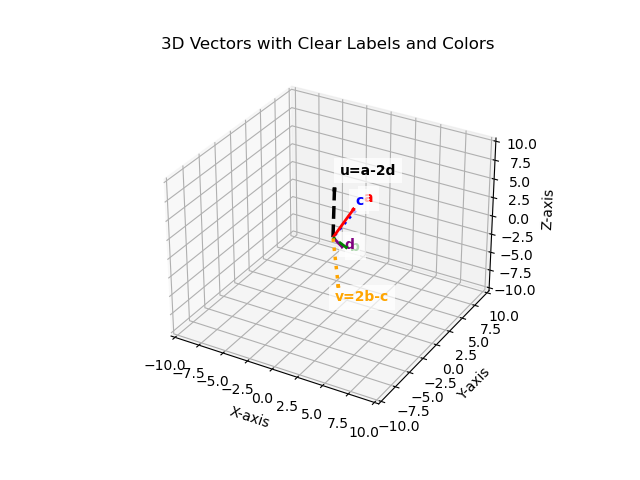
\includegraphics[width=0.9\columnwidth]{figs/fig4.png}
\caption{fig : Representation of vectors}
\label{Fig4}
\end{figure}
\end{frame}
\section{C Code}
\begin{frame}[fragile]
\frametitle{C Code }
\begin{lstlisting}[language=C]

#include <stdio.h>
#include <math.h>

// Function to check if (a-2d) is parallel to (2b-c)
int check_parallel(double a[3], double b[3], double c[3], double d[3]) {
    double u[3], v[3], cross[3];

    // u = a - 2d
    for (int i = 0; i < 3; i++) {
        u[i] = a[i] - 2.0 * d[i];
    }
    // v = 2b - c
    for (int i = 0; i < 3; i++) {
        v[i] = 2.0 * b[i] - c[i];
    }
\end{lstlisting}
\end{frame}
\begin{frame}[fragile]
\begin{lstlisting}
    // cross product u x v
    cross[0] = u[1]*v[2] - u[2]*v[1];
    cross[1] = u[2]*v[0] - u[0]*v[2];
    cross[2] = u[0]*v[1] - u[1]*v[0];

    // Check if cross product is (almost) zero
    double eps = 1e-9;
    if (fabs(cross[0]) < eps && fabs(cross[1]) < eps && fabs(cross[2]) < eps)
        return 1; // parallel
    else
        return 0; // not parallel
}
    
\end{lstlisting}
\end{frame}

\section{Python Code}
\begin{frame}[fragile]
\frametitle{Python : call\_c.py}
\begin{lstlisting}
import ctypes

# Load the shared library (make sure parallel.so is in the same folder)
lib = ctypes.CDLL("./parallel.so")

# Define argument and return types
lib.check_parallel.argtypes = [
    ctypes.POINTER(ctypes.c_double),  # a
    ctypes.POINTER(ctypes.c_double),  # b
    ctypes.POINTER(ctypes.c_double),  # c
    ctypes.POINTER(ctypes.c_double)   # d
]
lib.check_parallel.restype = ctypes.c_int

def check_parallel(a, b, c, d):
    """
    Calls the C function check_parallel(a, b, c, d).
    \end{lstlisting}
    \end{frame}
    \begin{frame}[fragile]
    \begin{lstlisting}
    Each of a, b, c, d must be length-3 lists or tuples.
    Returns True if (a-2d) || (2b-c), False otherwise.
    """
    # Convert Python lists to C arrays
    A = (ctypes.c_double * 3)(*a)
    B = (ctypes.c_double * 3)(*b)
    C = (ctypes.c_double * 3)(*c)
    D = (ctypes.c_double * 3)(*d)

    # Call the C function
    result = lib.check_parallel(A, B, C, D)
    return bool(result)

# ---------------- Example usage ----------------
if __name__ == "__main__":
    a = [1.0, 2.0, 3.0]
    b = [2.0, -1.0, 0.0]
\end{lstlisting}
\end{frame}
\begin{frame}[fragile]
\begin{lstlisting}
    c = [0.0, 4.0, 1.0]
    d = [1.0, 0.0, -1.0]
    
if check_parallel(a, b, c, d):
        print("(a - 2d) is parallel to (2b - c)")
    else:
        print("(a - 2d) is NOT parallel to (2b - c)")

\end{lstlisting}
\end{frame}

\begin{frame}[fragile]
\frametitle{Python Code for Plotting}
\begin{lstlisting}[language=Python]
import numpy as np
import matplotlib.pyplot as plt
from mpl_toolkits.mplot3d import Axes3D

def check_parallel(a, b, c, d, tol=1e-9):
    a, b, c, d = map(np.array, (a, b, c, d))
    u = a - 2*d
    v = 2*b - c
    cross = np.cross(u, v)
    return np.linalg.norm(cross) < tol, u, v

def plot_vectors(a, b, c, d, u, v):
    fig = plt.figure()
    ax = fig.add_subplot(111, projection='3d')
    # Helper function to draw vector + label
    def draw_vector(vec, name, color, style="-", scale=1.2, offset=(0,0,0), lw=2.0):
    \end{lstlisting}
    \end{frame}
    \begin{frame}[fragile]
    \begin{lstlisting}
        ax.quiver(0, 0, 0, vec[0], vec[1], vec[2],
                  color=color, linestyle=style,
                  arrow_length_ratio=0.08, linewidth=lw)
        ax.text(vec[0]*scale + offset[0],
                vec[1]*scale + offset[1],
                vec[2]*scale + offset[2],
                name, fontsize=10, weight="bold", color=color,
                bbox=dict(facecolor="white", alpha=0.7, edgecolor="none"))

    # Base vectors (unique colors + offsets to avoid overlap)
    draw_vector(a, "a", "red",    style="-",   offset=(0.4,  0.2, 0))
    draw_vector(c, "c", "blue",   style=":",   offset=(-0.4, -0.2, 0))
    draw_vector(b, "b", "green",  style="--",  offset=(0.3, -0.5, 0.3))   # shifted away
    draw_vector(d, "d", "purple", style="-.",  offset=(-0.3, 0.5, -0.3))  # opposite shift
\end{lstlisting}
\end{frame}
\begin{frame}[fragile]
\begin{lstlisting}
    # Special vectors u and v (thicker lines)
    draw_vector(u, "u=a-2d", "black",   style="--", lw=2.5, scale=1.25, offset=(0.3,0.3,0))
    draw_vector(v, "v=2b-c", "orange",  style=":",  lw=2.5, scale=1.25, offset=(-0.3,-0.3,0))

    # Axis scaling
    all_vecs = np.array([a, b, c, d, u, v])
    max_range = np.max(np.abs(all_vecs)) * 1.5 + 1
    ax.set_xlim([-max_range, max_range])
    ax.set_ylim([-max_range, max_range])
    ax.set_zlim([-max_range, max_range])

    ax.set_xlabel("X-axis")
    ax.set_ylabel("Y-axis")
    ax.set_zlabel("Z-axis")
    ax.set_title("3D Vectors with Clear Labels and Colors")
\end{lstlisting}
\end{frame}
\begin{frame}[fragile]
\begin{lstlisting}
    plt.show()

if __name__ == "__main__":
    a = np.array([1, 2, 3])
    b = np.array([2, -1, 0])
    c = np.array([0, 4, 1])
    d = np.array([1, 0, -1])

    is_parallel, u, v = check_parallel(a, b, c, d)
    print("Parallel?", is_parallel)

    plot_vectors(a, b, c, d, u, v)

\end{lstlisting}
\end{frame}

\end{document}
  